\documentclass[14pt]{extarticle} 
\usepackage{amsmath,mathtools,amsfonts,amsthm,amssymb,hyperref}
\usepackage{wasysym,geometry,bussproofs,latexsym,parskip,bookmark}
\usepackage{mathtools,float}
\newtheorem{defn}{Definition}
\newtheorem{thm}{Theorem}
\newtheorem{claim}{Claim}
\newtheorem{lemma}{Lemma}
\hypersetup{colorlinks,allcolors=blue,linktoc=all}
\geometry{a4paper} 
\geometry{margin=0.5in}
\title{Math for CS 2015/2019 solutions to ``In-Class Problems Week 7, Fri. (Session 17)''}
\author{https.//github.com/spamegg1}
\begin{document}
\maketitle
\tableofcontents

\section{Problem 1}
The table below lists some prerequisite information for some subjects in the MIT Computer Science program (in 2006). This defines an indirect prerequisite relation that is a DAG with these subjects as vertices.

\begin{center}
\begin{tabular}{ll}
$18.01 \to 6.042$ & $18.01 \to 18.02$ \\
$18.01 \to 18.03$ & $6.046 \to 6.840$ \\
$8.01 \to 8.02$ & $6.001 \to 6.034$ \\
$6.042 \to 6.046$ & $18.03, 8.02 \to 6.002$ \\
$6.001, 6.002 \to 6.003$ & $6.001, 6.002 \to 6.004$ \\
$6.004 \to 6.033$ & $6.033 \to 6.857$
\end{tabular}
\end{center}

\subsection{(a)}
Explain why exactly six terms are required to finish all these subjects, if you can take as many subjects as you want per term. Using a greedy subject selection strategy, you should take as many subjects as possible each term. Exhibit your complete class schedule each term using a greedy strategy.

\begin{proof}
It helps to have a diagram of the direct prerequisite relation:

\begin{figure}[ht!]
\centering
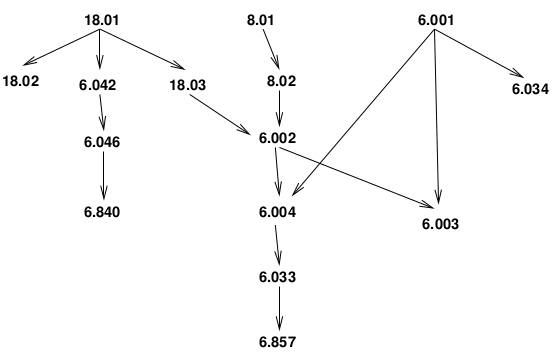
\includegraphics[scale=0.75]{prereq.png}
\end{figure}

There is a chain of length 6:

$8.01 \to 8.02 \to 6.002 \to 6.004 \to 6.033 \to 6.857$

So we need at least 6 terms. 

So six terms are necessary, because at most one of these subjects can be taken each term.

There is no longer chain than length 6, so with the greedy strategy you will take six terms. Here are the subjects you take in successive terms.

Here's a greedy schedule:

Term 1: take 6.001, 8.01, 18.01, 

Term 2: take 6.034, 6.042, 8.02, 18.02, 18.03, 

Term 3: take 6.002, 6.046,

Term 4: take 6.003, 6.004, 6.840,

Term 5: take 6.033,

Term 6: take 6.857.
\end{proof}

\subsection{(b)}
In the second term of the greedy schedule, you took five subjects including 18.03. Identify a set of five subjects not including 18.03 such that it would be possible to take them in any one term (using some nongreedy schedule). Can you figure out how many such sets there are?

\begin{proof}
Here are all the chains:

$$
\begin{array}{cccccccc}
18.01 & 18.01 & 18.01 & 18.01 & 6.001 & 6.001 & 8.01 & 8.01 \\
\downarrow & \downarrow  & \downarrow & \downarrow & \downarrow & \downarrow & \downarrow & \downarrow \\
6.042 & 18.02 & 18.03 & 18.03 & 6.003 & 6.034 & 8.02 & 8.02 \\
\downarrow &   & \downarrow & \downarrow & & & \downarrow & \downarrow \\
6.046 & & 6.002 & 6.002 & & & 6.002 & 6.002 \\
\downarrow &   & \downarrow & \downarrow & & & \downarrow & \downarrow \\
6.840 & & 6.003 & 6.004 & & & 6.003 & 6.004 \\
& &  & \downarrow &  &  &  & \downarrow \\
& & & 6.033 & & & & 6.033\\
& & & \downarrow &  &  &  & \downarrow \\
& & & 6.857 & & & & 6.857
\end{array}
$$

We're looking for an antichain that does not include 18.03. Every such antichain will have to include 18.02, 6.003, 6.034. Then a fourth subject could be any of 6.042, 6.046, and 6.840. The fifth subject could then be any of 6.004, 6.033, and 6.857. This gives a total of nine antichains of five subjects.
\end{proof}

\subsection{(c)}
Exhibit a schedule for taking all the courses - but only one per term.
\begin{proof}
We're asking for a topological sort. There are many. One is: 

18.01, 8.01, 6.001, 18.02, 6.042, 18.03, 8.02, 6.034, 6.046, 6.002, 6.840, 6.004, 6.003, 6.033, 6.857.
\end{proof}

\subsection{(d)}
Suppose that you want to take all of the subjects, but can handle only two per term. Exactly how many terms are required to graduate? Explain why.
\begin{proof}
There are $\lceil15/2\rceil = 8$ terms necessary. The schedule below shows that 8 terms are sufficient as well:

\begin{center}
\begin{tabular}{lcc}
1: & 18.01 & 8.01\\
2: & 6.001 & 18.02\\
3: & 6.042 & 18.03\\
4: & 8.02 & 6.034\\
5: & 6.046 & 6.002\\
6: & 6.840 & 6.004\\
7: & 6.003 & 6.033\\
8: & 6.857
\end{tabular}
\end{center}
\end{proof}

\subsection{(e)}
What if you could take three subjects per term?
\begin{proof}
From part (a) we know six terms are required even if there is no limit on the number of subjects per term. Six terms are also sufficient, as the following schedule shows:

\begin{center}
\begin{tabular}{lccc}
1: & 18.01 & 8.01 & 6.001 \\
2: & 6.042 & 18.03 & 8.02 \\
3: & 18.02 & 6.046 & 6.002 \\
4: & 6.004 & 6.003 & 6.034 \\
5: & 6.840 & 6.033 &\\
6: & 6.857 &  &
\end{tabular}
\end{center}
\end{proof}

\section{Problem 2}
A pair of Math for Computer Science Teaching Assistants, Lisa and Annie, have decided to devote some of their spare time this term to establishing dominion over the entire galaxy. Recognizing this as an ambitious project, they worked out the following table of tasks on the back of Annie’s copy of the lecture notes.

1. Devise a logo and cool imperial theme music - 8 days.

2. Build a fleet of Hyperwarp Stardestroyers out of eating paraphernalia swiped from Lobdell - 18 days.

3. Seize control of the United Nations - 9 days, after task \#1.

4. Get shots for Lisa’s cat, Tailspin - 11 days, after task \#1.

5. Open a Starbucks chain for the army to get their caffeine - 10 days, after task \#3.

6. Train an army of elite interstellar warriors by dragging people to see The Phantom Menace dozens of times - 4 days, after tasks \#3, \#4, and \#5.

7. Launch the fleet of Stardestroyers, crush all sentient alien species, and establish a Galactic Empire - 6 days, after tasks \#2 and \#6.

8. Defeat Microsoft - 8 days, after tasks \#2 and \#6.

We picture this information in Figure 1 below by drawing a point for each task, and labelling it with the name and weight of the task. An edge between two points indicates that the task for the higher point must be completed before beginning the task for the lower one.

\begin{figure}[ht!]
\centering
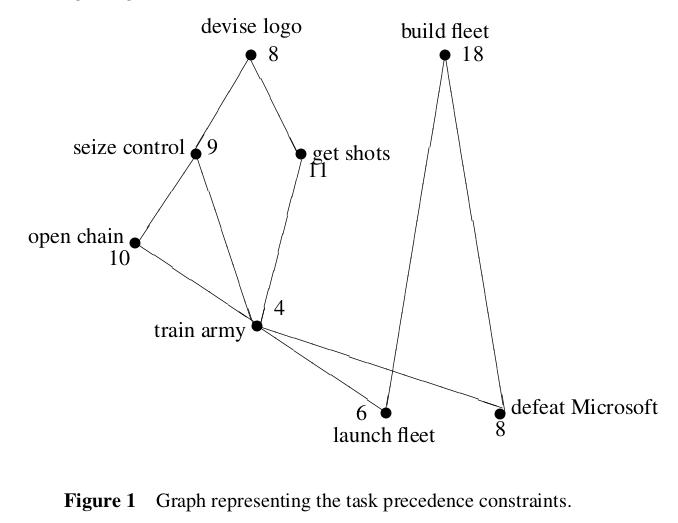
\includegraphics[scale=0.5]{precedence.png}
\end{figure}

\subsection{(a)}
Give some valid order in which the tasks might be completed.
\begin{proof}
We can easily find several of them. The most natural one is valid, too: \#1, \#2, \#3, \#4, \#5, \#6, \#7, \#8.
\end{proof}

Lisa and Annie want to complete all these tasks in the shortest possible time. However, they have agreed on some constraining work rules.

Only one person can be assigned to a particular task; they cannot work together on a single task.

Once a person is assigned to a task, that person must work exclusively on the assignment until it is completed. So, for example, Lisa cannot work on building a fleet for a few days, run to get shots for Tailspin, and then return to building the fleet.

\subsection{(b)}
Lisa and Annie want to know how long conquering the galaxy will take. Annie suggests dividing the total number of days of work by the number of workers, which is two. What lower bound on the time to conquer the galaxy does this give, and why might the actual time required be greater?
\begin{proof}
$$
\frac{8+18+9+11+10+4+6+8}{2} = 37 \text{ days}
$$

If working together and interrupting work on a task were permitted, then this answer would be correct. However, the rules may prevent Lisa and Annie from both working all the time. For example, suppose the only task was building the fleet. It will take 18 days, not 18/2 days, to complete, because only one person can work on it and the other must sit idle.
\end{proof}

\subsection{(c)}
Lisa proposes a different method for determining the duration of their project. She suggests looking at the duration of the critical path, the most time-consuming sequence of tasks such that each depends on the one before. What lower bound does this give, and why might it also be too low?
\begin{proof}
The longest sequence of tasks is devising a logo (8 days), seizing the U.N. (9 days), opening a Starbucks (10 days), training the army (4 days), and then defeating Microsoft (8 days). Since these tasks must be done sequentially, galactic conquest will require at least 39 days.

If there were enough workers, this answer would be correct; however, with only two workers, Lisa and Annie may be unable to make progress on the critical path every day. For example, suppose
there were only four tasks: devise logo, build fleet, seize control, get shots. Now the critical path consists of two critical tasks: devise logo, get shots, which take 19 days. But to get through this path in 19 days, some worker must be working on a critical task at all times for the 19 days. This leaves only one worker free to complete building the fleet and seizing control, which will take at least 27 days. So in fact, 27 days is the minimum time for two workers to complete these four tasks.
\end{proof}

\subsection{(d)}
What is the minimum number of days that Lisa and Annie need to conquer the galaxy? No proof is required.
\begin{proof}
40 days. Tasks could be divided as follows:

Annie: \#1 (days 1-8), \#3 (days 9-17), \#4 (days 18-28), \#8 (days 33-40).

Lisa: \#2 (days 1-18), \#5 (days 19-28), \#6 (days 29-32), \#7 (days 33-38).

It takes some care to verify that 40 days is the best you can do. If someone comes up with a simple proof of this, tell the course staff.
\end{proof}

\section{Problem 3}
Sauron finds that conquering Middle Earth breaks down into a bunch of tasks. Each task can be completed by a horrible creature called a Ringwraith in exactly one week. Sauron realizes the prerequisite structure among the tasks defines a DAG. He has $n$ tasks in his DAG, with a maximum length chain of $t$ tasks.

\subsection{(a)}
Sauron is trying to describe various features of his scheduling problem using standard terminology. For each feature below, indicate the number of the corresponding term.

\begin{center}
{\bf Standard Terminology}
\begin{tabular}{llll}
1. & Indirect prerequisite & 2. & Topological sort \\
3. & Chain & 4. & Antichain \\
5. & Size of the largest antichain & 6. & Size of the smallest antichain \\
7. & Length of the longest chain & 8. & Length of the shortest chain \\
\end{tabular}
\end{center}

\begin{tabular}{ll}
1. & A set of tasks that can be worked on simultaneously. \\

2. & A possible order in which all the tasks could be completed, \\

& if only one Ringwraith were available. \\

3. & The minimum number of weeks required to complete all tasks, \\
& if an unlimited number of Ringwraiths were available.
\end{tabular}

\begin{proof}
1. (4) An antichain. 2. (2) Topological sort. 3. (7) Length of the longest chain.
\end{proof}

\subsection{(b)}
If Sauron is lucky, he will be able to get away with a small crew of Ringwraiths. Write a simple formula involving $n$ and $t$ for the smallest number of Ringwraiths that could possibly be able to complete all $n$ tasks in $t$ weeks. (Do not make any additional assumptions about the relative sizes of $n$ and $t$ besides $t \leq n$.) Given any $n$ and $t$, describe a DAG that can be completed in $t$ weeks using this number of Ringwraiths.
\begin{proof}
If $t = n$ and the whole DAG is a single chain, then only 1 Ringwraith is needed, since no tasks can be parallelized.

More generally, for any $1 \leq t \leq n$, the smallest number of Ringwraiths needed corresponds to the situation of minimum parallelizability; in other words, having as long chains as possible.

If the DAG consists entirely of exactly max length ($t$) chains (maybe with the exception of the last one, which might end up shorter than $t$ if $n$ is not a multiple of $t$), then there are $\displaystyle\left\lceil \frac{n}{t} \right\rceil$ chains, each of which requires 1 Ringwraith, so the smallest number of Ringwraiths is $\displaystyle\left\lceil \frac{n}{t} \right\rceil$.
\end{proof}

\subsection{(c)}
On the other hand, if Sauron is unlucky, he may need a large crew of Ringwraiths in order to conquer Middle Earth in $t$ weeks. Write a simple formula involving $n$ and $t$ for the largest number of Ringwraiths that Sauron would ever need in order to be sure of completing all $n$ tasks in $t$ weeks - no matter how unlucky he was. Given any $n$ and $t$, describe a DAG that can be completed in $t$ weeks and requires this number of Ringwraiths.
\begin{proof}
Since there is a maximum length chain of $t$ tasks, there is AT LEAST one chain of length $t$. Having more such chains reduces the number of Ringwraiths as in part (b), so the worst case is when all the other remaining $n-t$ tasks form an antichain.

Consider the DAG of $n$ tasks, where $t$ of these tasks form a prerequisite chain, and the remaining $n-t$ tasks are incomparable to each other (each single task is a length-1 chain by itself) and to the chain (i.e. an antichain). Then the length $t$ chain requires 1 Ringwraith, and the other $n-t$ tasks can be parallelized, each requiring 1 Ringwraith, for a total of $n-t+1$ Ringwraiths.
\end{proof}

\section{Problem 4}
If $a$ and $b$ are distinct nodes of a digraph, then $a$ is said to {\it cover} $b$ if there is an edge from $a$ to $b$ and every path from $a$ to $b$ includes this edge. If $a$ covers $b$, the edge from $a$ to $b$ is called a {\it covering edge}.
\subsection{(a)}
What are the covering edges in the DAG in Figure 2?
\begin{figure}[ht!]
\centering
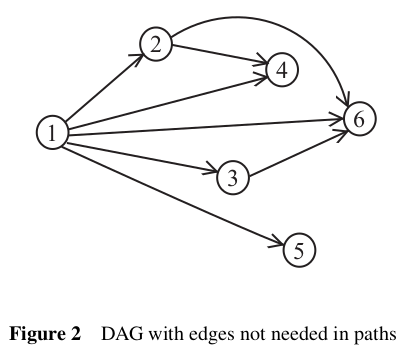
\includegraphics[scale=0.5]{dag.png}
\end{figure}

\begin{proof}
$1 \to 2$ is a covering edge, because it's the only path from 1 to 2.

$1 \to 3$ is a covering edge, because it's the only path from 1 to 3.

$1 \to 4$ is not a covering edge, because there is another path $1 \to 2 \to 4$ from 1 to 4 which doesn't include it.

$1 \to 5$ is a covering edge, because it's the only path from 1 to 5.

$1 \to 6$ is not a covering edge, because there is another path $1 \to 3 \to 6$ from 1 to 6 which doesn't include it.

Similarly $2 \to 4$, $2 \to 6$ and $3 \to 6$ are all covering edges.
\end{proof}

\subsection{(b)}
Suppose $D$ is a finite DAG. Let $covering(D)$ be the subgraph of $D$ consisting of only the covering edges. Explain why $covering(D)$ has the same positive walk relation as $D$.

Hint: Consider longest paths between a pair of vertices.
\begin{proof}
1. We need to show that if there is a path in $D$ between vertices $a \neq b$, then there is a path consisting only of covering edges from $a$ to $b$. (This will prove that $D$ and $(D)$ have the same positive walk relation.)

2. Since $D$ is a finite DAG, there must be a longest path $P$ from $a$ to $b$. (The path length is bounded above by the number of edges in $D$.)

3. Now every edge on this path $P$ must be a covering edge or it could be replaced by a path of length 2 or more, yielding a longer path from $a$ to $b$.
\end{proof}

\subsection{(c)}
Show that if two DAG's have the same positive walk relation, then they have the same set of covering edges.
\begin{proof}
1. Suppose $C$ and $D$ are DAG’s with the same positive walk relation and that $a \to b$ is a covering edge of $C$. 

2. We want to show that $a \to b$ must also be a covering edge of $D$.

3. Since $a \to b$ itself defines a (length 1) positive length path in $C$, there must be a positive length path $P$ in $D$ from $a$ to $b$. 

4. If $P$ has length greater than 1, then $P$ must consist of a positive length path $P_1$ from $a$ to $c$, followed by a positive length path $P_2$ from $c$ to $b$, for some vertex, $c$. 

5. Also, since $D$ is a DAG, c cannot be $a$ or $b$.

6. By (4) and (5) there must also be positive length paths $Q_1$ in $C$ from $a$ to $c$ and $Q_2$ from $c$ to $b$, and neither of these paths can traverse $a \to b$ or there would be a cycle. 

7. Hence the path $Q_1 + Q_2$ from $a$ to $c$ to $b$ is a path in $C$ that does not traverse $a \to b$, contradicting the fact that $a \to b$ is a covering edge of $C$.

8. In summary, there is a length 1 path from $a$ to $b$ in $D$, namely $a \to b$, and this is the only path from $a$ to $b$ in $D$, which proves that $a \to b$ is a covering edge in $D$.
\end{proof}

\subsection{(d)}
Conclude that covering $(D)$ is the unique DAG with the smallest number of edges among all digraphs with the same positive walk relation as $D$.
\begin{proof}
1. By part (c), any DAG with the same positive walk relation as $D$ must contain all the edges of $covering(D)$. 

2. By part (b), $covering(D)$ has this same positive walk relation. It follows immediately that $covering(D)$ is the unique minimum-size DAG with the same positive path relation as $D$.
\end{proof}

The following examples show that the above results don't work in general for digraphs with cycles.

\subsection{(e)}
Describe two graphs with vertices $\{1, 2\}$ which have the same set of covering edges, but not the same positive walk relation. (Hint: Self-loops.)
\begin{proof}
1. Let one graph $G$ have edges $\{(1, 2), (1, 1)\}$ and the other graph $H$ have edges $\{(1, 2), (2, 2)\}$. 

2. $G$ and $H$ have the same set of covering edges, namely, $(1, 2)$. 

3. But in $H$ there is a positive length path from 2 to 2, namely a path of length 1, but there is no positive length path from 2 to 2 in $G$.
\end{proof}

\subsection{(f)}
(i) The {\it complete digraph} without self-loops on vertices 1, 2, 3 has edges between every two distinct vertices. What are its covering edges?

(ii) What are the covering edges of the graph with vertices 1, 2, 3 and edges $\langle 1 \to 2 \rangle, \langle 2 \to 3 \rangle, \langle 3 \to 1\rangle$?

(iii) What about their positive walk relations?
\begin{proof}
(i) There are no covering edges, since there is always a length 2 path from $a$ to $b$ that does not use the edge $a \to b$.

(ii) All three edges are the covering edges.

(iii) They have the same positive walk relation, namely, each vertex is connected to all the vertices, including itself, by positive length paths.
\end{proof}
\end{document}
